\documentclass[a4paper,11pt]{article}
\usepackage{graphicx}
\usepackage{a4wide}
\usepackage{hyperref}
\usepackage{times}
\usepackage[francais]{babel}
\usepackage[utf8]{inputenc}

\usepackage[compact]{titlesec}  
%\titlespacing{\section}{0pt}{0pt}{0pt}
\titlespacing{\subsection}{0pt}{.8em}{.4em}
\setlength\belowcaptionskip{0.200ex}
\setlength\abovecaptionskip{0.050ex}
\setlength\intextsep{2ex}
\setlength\textfloatsep{2ex}
\setlength\floatsep{0.05ex}
\setlength\topmargin{-15mm}
\addtolength\textheight{10mm}
\renewcommand{\baselinestretch}{0.97}

%\author{Pascal Lafourcade \and Gilles Mounier \and Benjamin Wack}
\title{Introduction \`a l'algorithmique \\ avec le jeu Cargo-Bot}
%\includegraphics[width =1cm]{cargo-bot-icon.png}

\graphicspath{{imgweb/}}

\date{}%17 mars 2014}
\pagestyle{empty}

\begin{document}

\maketitle
\thispagestyle{empty}
\vspace{-6cm} \hspace*{12.5cm}  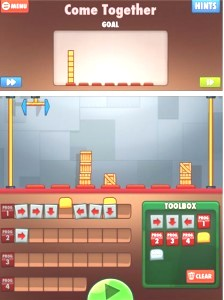
\includegraphics[width = 4 cm]{cargo-bot-screen}


\section*{Pour jouer chez soi}

{\Large\url{http://www-verimag.imag.fr/~wack/CargoBot/}}

\medskip

Attention, ce site ne fonctionne pas sur les anciennes versions
d'Internet Explorer. On peut installer le navigateur Firefox, ou si on
veut un logiciel plus léger, QtWeb (\url{http://qtweb.net}).

\section*{Qu'apprend-on en jouant à Cargo-Bot ?}

Lorsqu'on a trouvé une solution à un niveau, on a écrit un
\emph{algorithme} pour le résoudre : une méthode qui marche à tous les
coups pour arriver au résultat voulu. La grue n'a alors plus qu'à
\emph{exécuter} cet algorithme, c'est-à-dire faire exactement ce qu'on
lui dit. En revanche, elle n'a pas besoin de \og comprendre \fg{} ce
qu'elle fait pour le faire correctement.

\subsection*{Suite d'instructions}
\vspace{-2mm}
Un algorithme, la plupart du temps, est constitué d'instructions
très simples (ici 
\includegraphics[width
=.5cm]{left}, 
\includegraphics[width =.5cm]{right}
et 
\includegraphics[width=0.5cm]{down}) que l'on place l'une à la
suite de l'autre et qu'on doit exécuter \emph{dans l'ordre} où elles
sont écrites.

\subsection*{Les programmes}

Ce qui est un peu moins courant ici, c'est qu'on écrit non pas un mais
quatre programmes, qui peuvent ensuite s'\emph{appeler} les uns les
autres. Cela permet de regrouper dans un programme une suite
d'instructions particulière (par exemple qui déplace un cube d'un cran
vers la droite), puis d'appeler ce programme plusieurs fois (pour
déplacer plusieurs cubes). On crée ainsi une sorte de boucle.

%Il existe des langages de programmation qui sont construits presque
%uniquement avec ce mécanisme.

\subsection*{Un programme qui s'appelle lui-même}

Si on veut déplacer toute une pile de cubes vers la droite, au lieu de
r\'ep\'eter plusieurs fois l'appel à un programme, il est plus
\'economique d'\'ecrire un programme qui signifie
\og Déplace un cube vers la droite et recommence \fg{}. De plus ce
programme fonctionnera quelle que soit la taille de la pile à
déplacer. C'est possible si on écrit un programme qui s'appelle lui-m\^eme.

Attention, un tel programme ne s'arrêtera jamais de lui-même ! Ici
cela fonctionne car le jeu s'arrête dès qu'on est arrivé dans la
situation gagnante.

\subsection*{Pour aller plus loin}

Ceux qui ont déjà des notions d'algorithmique auront peut-être
remarqué qu'il n'y a pas de variable dans les programmes qu'on
écrit. Il existe cependant une forme de \og mémoire \fg{} dans ce jeu
: la position des cubes à un moment donné.

% \subsection*{Conditions}

Dans les niveaux plus avancés, il existe également des \'etiquettes
qui permettent de ne faire une action que si la grue contient un
certain cube. Cela permet par exemple de trier les cubes en fonction
de leur couleur, mais aussi d'écrire des programmes très sophistiqués
qui divisent une pile de cube en deux, qui rassemblent tous les cubes
au même endroit, etc.


\section*{Rappel des règles du jeu}


\subsection*{Présentation et but du jeu}

Ce jeu consiste \`a programmer une grue qui manipule des containers,
symbolisés par des cubes de couleurs diff\'erentes : Rouge
%
\includegraphics[width =.5cm]{Redbox}
, Jaune %
\includegraphics[width =.5cm]{Yellowbox}
, Vert %
\includegraphics[angle = 90, width =.5cm]{Greenbox}
et Bleu
%
\includegraphics[width =.5cm]{Bluebox}
.

L'écran de jeu est divisé en trois zones :
\begin{itemize}
\item En haut, le but à atteindre. \textbf{Dès que les cubes sont dans
  cette position, c'est gagné !}
\item Au milieu, le terrain de jeu proprement dit, avec la position de
  départ des cubes et la grue qui permet de les déplacer.
\item En bas, la zone de programme où on fait glisser des
  instructions (
\includegraphics[width
  =.5cm]{left} 
\includegraphics[width
  =.5cm]{right} 
\includegraphics[width=0.5cm]{down} 
\includegraphics[width
  =.5cm]{f0} 
\includegraphics[width=.5cm]{f1}
  
\includegraphics[width=.5cm]{f2} 
\includegraphics[width=.5cm]{f3})
% pour former des programmes.
\end{itemize}

Une fois un programme écrit, on peut l'exécuter en cliquant sur
\texttt{Play}, recommencer avec \texttt{Rewind}, modifier la vitesse
d'exécution, etc.

\medskip

Tout en haut de l'écran, on dispose également de menus déroulants pour
choisir les niveaux à résoudre. Ils sont organisés par groupes de 6 et
classés par ordre de difficulté croissante.
% Il est bien sûr conseillé
% de commencer par \og Tutorial 1 \fg{}, puis \og Tutorial 2 \fg...

\subsection*{Déplacements}
\vspace{-0.2cm}

Il est toujours possible de d\'eplacer la grue vers la droite ou vers
la gauche \emph{à condition de ne pas sortir du terrain de jeu}.
%
La flèche 
\includegraphics[width=0.5cm]{down} peut avoir trois
effets différents :
\begin{itemize}
\item Si la pince est vide et qu'il y a un cube en dessous, elle
  le saisit et remonte.
\item Si la pince est vide et qu'il n'y a pas de cube en dessous, elle
  descend et remonte \`a vide.
\item Si la pince contient un cube, elle le d\'epose et remonte
  \`a vide.
\end{itemize}


\subsection*{Programmes}

Chaque programme (F0, F1, F2, F3) est constitué de 8 instructions au
maximum, sauf le dernier qui est limité à 5.
Il n'y a pas de \og retour à la ligne \fg{} automatique : une fois
qu'un programme est fini, il ne se passe plus rien !



Les instructions 
\includegraphics[width
=.5cm]{f0},  
\includegraphics[width=.5cm]{f1}... permettent
d'\emph{appeler} un programme : on quitte (temporairement) le programme
en cours, on va exécuter celui désigné par cette instruction, puis on
revient au programme de départ s'il n'était pas fini.


\subsection*{\'Etiquettes   
\includegraphics[width =.5cm]{red} 
\includegraphics[width
    =.5cm]{yellow} 
\includegraphics[width =.5cm]{green}
 
\includegraphics[width =.5cm]{blue}
}

Elles ne sont disponibles que dans les niveaux plus avancés. On les
place au-dessus d'une instruction, et cette instruction ne s'effectue
que si la pince contient un cube de la bonne couleur.
% ( 
\includegraphics[width =.5cm]{red}, 
\includegraphics[width
%    =.5cm]{yellow}, 
\includegraphics[width =.5cm]{green},
%  ou 
\includegraphics[width =.5cm]{blue}).

Il y a aussi une \'etiquette
  repr\'esentant {\it toutes les couleurs} 
\includegraphics[width
    =.5cm]{any} qui effectue une instruction seulement si
  la pince contient un cube (ind\'ependemment de sa couleur), et
  une autre \'etiquette {\it vide} 
\includegraphics[width
    =.5cm]{none} qui n'ex\'ecute l'instruction que si la pince est
  vide.


\subsection*{Score}

Le jeu attribue entre 0 et 3 étoiles à une solution, en fonction du
\emph{nombre d'instructions} qu'elle comporte : la solution la plus
courte possible rapportera 3 étoiles.
%
Attention, on rend parfois un programme complètement incompréhensible
à force de vouloir le raccourcir !

\end{document}
